\chapter{Results}
\label{chapter:results}

  The main focus of this thesis is to present a proof-of-concept caching
  algorithm that is based on statistical foundations rather than on heuristics.
  In order to confirm that MMC makes reasonable decisions, I wrote a
  caching simulator in Python2 that accepts a sequence of page requests and
  then uses the equations derived in chapter \ref{chapter:methods} to decide
  whether to evict a page or to purge all metadata for a page. I compared this
  to the hit-rate performance achieved with similarly sized caches using the
  LRU, ARC, and MIN policies. I used the SPC1 traces hosted by the University of
  Massachusetts \cite{SPC1} to test the algorithms. All code used to produce
  results reported in this thesis is available open-source on a GitHub
  repository \cite{supplimental}.

  Several challenges need to be addressed before the MMC algorithm is ready for
  a production environment; benchmarking the algorithm before that point would
  be premature. Many of those challenges are outlined in section
  \ref{chapter:future_work}.

  However, the preliminary results suggest that MMC vastly outperforms the
  least-recently used (LRU) algorithm and compares favorably to the adaptive
  replacement cache (ARC) algorithm. I used the two OLTP traces named
  Financial1.spc and Financial2.spc, published by the Storage Performance Council
  and the University of Massachusetts \cite{SPC1, OLTPtraces}. These are
  examples of a financial database work flow, but they should not be interpreted
  as being representative of financial database work flows or of computing
  work flows in general.

  These two traces record roughly 30 million transactions of 512KB pages, which
  works out to a little over a terabyte of data requested per hour. In order to
  create manageable graphs, I have broken these traces into smaller segments.
  The stack depth distribution for the first million page request for the files
  Financial1.spc and Financial2.spc is shown in Figure \ref{fig:sdd_financial1}
  and the cumulative stack depth distribution is shown in Figure
  \ref{fig:sdd_cdf_financial1}.

  \begin{figure}
  \centering
  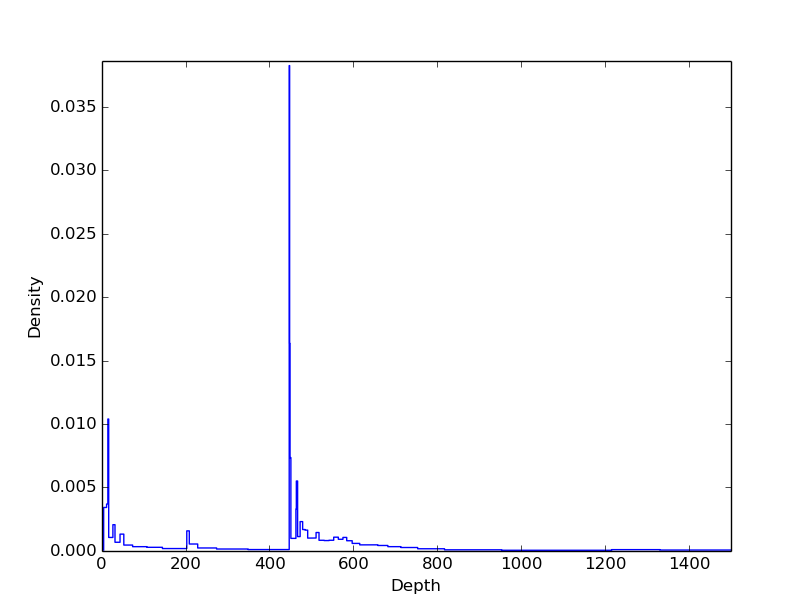
\includegraphics[width=6in]{../media/sdd_financial1_0-1000000.png}
  \caption[SDD of trace Financial1.spc]{This shows the stack depth distribution
  (SDD) for the first 1000000 page requests from Financial1.spc.}
  \label{fig:sdd_financial1}
  \end{figure}

  \begin{figure}
  \centering
  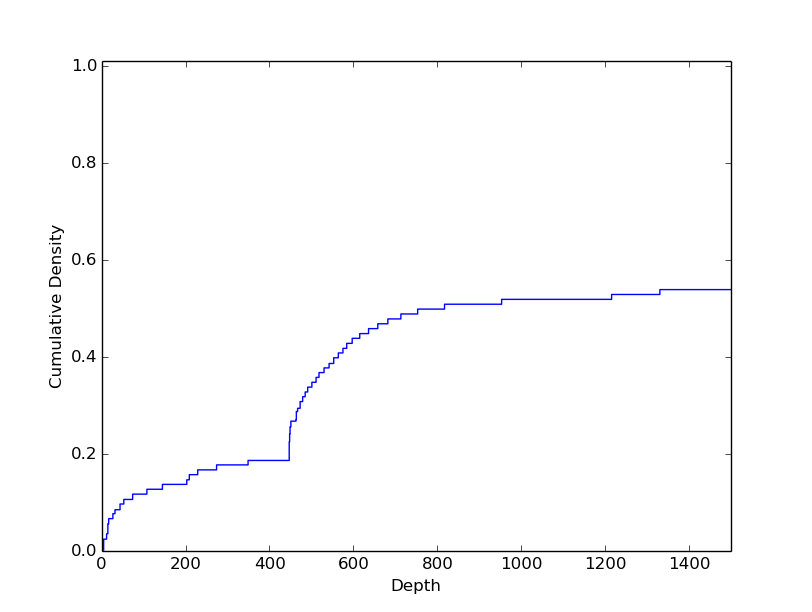
\includegraphics[width=6in]{../media/sdd_cdf_financial1_0-1000000.png}
  \caption[CDF for the SDD of trace Financial1.spc]{This is the cumulative
  distribution function for the stack depth distribution for the first 1000000
  page requests from Financial1.spc. The cumulative value at a depth of 445 is
  12.7\%.}
  \label{fig:sdd_cdf_financial1}
  \end{figure}

  This suggests a few interesting test cases. If we choose a cache size of
  445, the LRU will completely miss the second high density region and the hit
  rate will be limited to $12.7\%$. A good algorithm will be able to identify
  enough important pages that it can cache many of the pages that are only
  referenced again after their depth in the stack depth distribution exceeds
  445. This represents a cache that can only hold 222.5 MB.

  It is worth noting that the bimodality of Figure \ref{fig:sdd_financial1} does
  not indicate that a geometric distribution is a poor model for the stack depth
  distribution. MMC has enough degrees of freedom that it can instead assign
  page requests from the second high density region to the independent reference
  model.

  In order compare how well MMC performs, I created several time-series graphs,
  shown in Figures \ref{fig:ts_445_financial1}, \ref{fig:ts_600_financial1},
  \ref{fig:ts_1000_financial1}, \ref{fig:ts_445_financial2},
  \ref{fig:ts_600_financial2}, and
  \ref{fig:ts_1000_financial2} that chart the cumulative average
  and the rolling average for MMC, LRU, ARC, and MIN.

  \begin{figure}
  \centering
  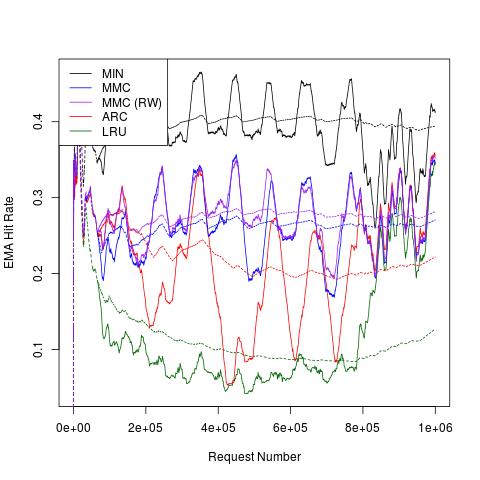
\includegraphics[width=6in]{../media/ts_445_445_1780_2.png}
  \caption[Rolling hit rate for 445 page caches on trace Financial1.spc]{This
  shows the average hit rates (dotted lines) and exponential moving average hit
  rates (solid lines) for several algorithms on the first 1000000 page requests
  in Financial1.spc. The cache size is 445, which is specifically picked because
  the SDD has a high density region starting at a depth of 446. This causes the
  LRU to evict a large number of pages just before they will be requested again.
  The ARC algorithm uses a heuristic that causes it to act like an LRU for large
  portions of this trace. The LRU would have needed to be 11\% longer to achieve
  the same hit rate as ARC and 31\% longer to achieve the same hit rate as
  MMC(RW), which includes the distinction of whether the last reference to a
  page was a read or a write.}
  \label{fig:ts_445_financial1}
  \end{figure}

  \begin{figure}
  \centering
  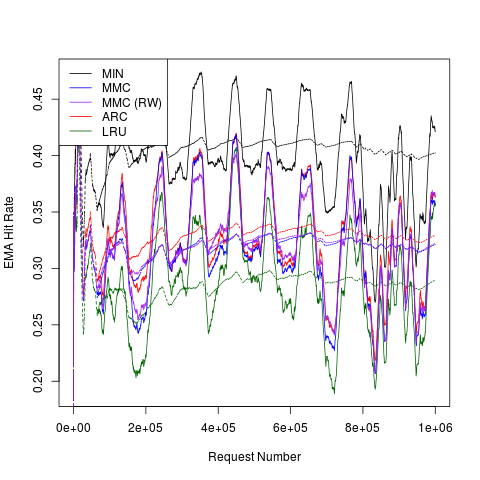
\includegraphics[width=6in]{../media/ts_600_600_2400_2.png}
  \caption[Rolling hit rate for 600 page caches on trace Financial1.spc]{This
  shows the average hit rates (dotted lines) and exponential moving average hit
  rates (solid lines) for several algorithms on the first 1000000 page requests
  in Financial1.spc. The cache size is 600. In certain areas, the hit rates for
  all of the compared algorithms plummets. In these areas, the trace is
  exhibiting the type of behavior expected from a file scan. While the ARC
  algorithm has the best performance on this trace, the MMC algorithms do well
  in the periods just after a file scan. The size of the cache would need to
  have been increased by 26\% for the LRU to achieve the same hit rate as ARC
  and 19\% to match MMC(RW).}
  \label{fig:ts_600_financial1}
  \end{figure}

  \begin{figure}
  \centering
  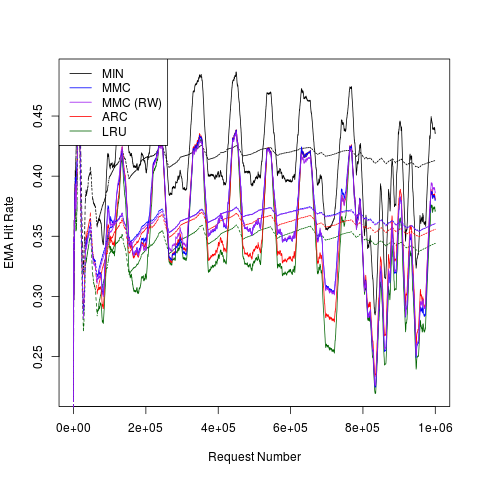
\includegraphics[width=6in]{../media/ts_1000_1000_4000_2.png}
  \caption[Rolling hit rate for 1000 page caches on trace Financial1.spc]{This
  shows the average hit rates (dotted lines) and exponential moving average hit
  rates (solid lines) for several algorithms on the first 1000000 page requests
  in Financial1.spc. The cache size is 1000.}
  \label{fig:ts_1000_financial1}
  \end{figure}

  \begin{figure}
  \centering
  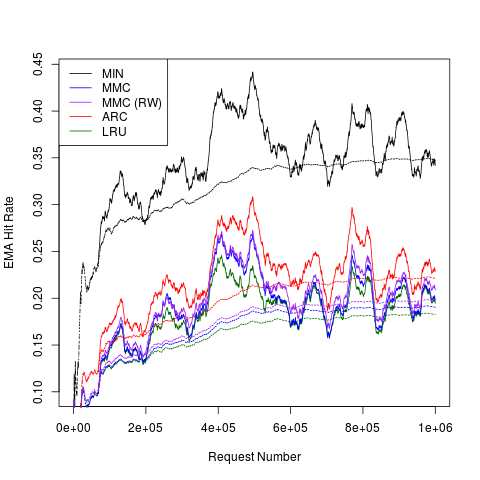
\includegraphics[width=6in]{../media/ts_445_445_1780_3.png}
  \caption[Rolling hit rate for 445 page caches on trace Financial2.spc]{This
  shows the average hit rates (dotted lines) and exponential moving average hit
  rates (solid lines) for several algorithms on the first 1000000 page requests
  in Financial2.spc. The cache size is 445. The LRU cache would need to be 14\%
  larger to have the same hit rate as MMC, 27\% larger to match the hit rate of
  MMC with read/write information, and 83\% larger to match ARC.}
  \label{fig:ts_445_financial2}
  \end{figure}

  \begin{figure}
  \centering
  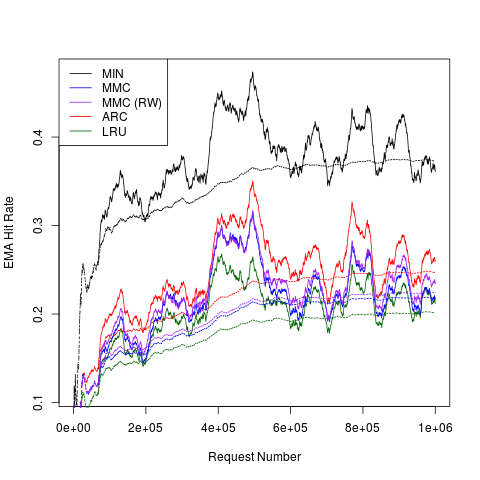
\includegraphics[width=6in]{../media/ts_600_600_2400_3.png}
  \caption[Rolling hit rate for 600 page caches on trace Financial2.spc]{This
  shows the average hit rates (dotted lines) and exponential moving average hit
  rates (solid lines) for several algorithms on the first 1000000 page requests
  in Financial2.spc. The cache size is 600. The hit rate for MMC is equivalent
  to a 28\% larger LRU. MMC with read/write information has the same hit rate as
  a 41\% larger LRU. ARC has the same hit rate as a 90\% larger LRU.}
  \label{fig:ts_600_financial2}
  \end{figure}

  \begin{figure}
  \centering
  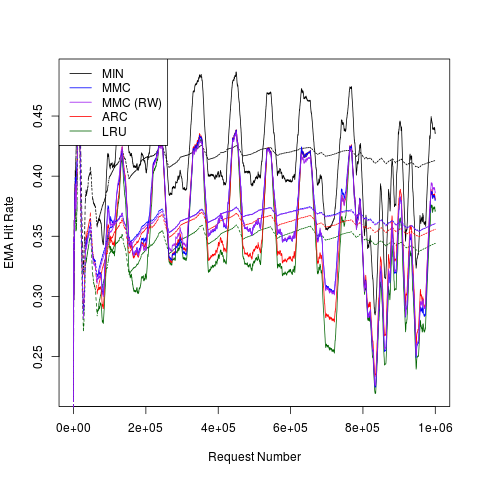
\includegraphics[width=6in]{../media/ts_1000_1000_4000_2.png}
  \caption[Rolling hit rate for 1000 page caches on trace Financial2.spc]{This
  shows the average hit rates (dotted lines) and exponential moving average hit
  rates (solid lines) for several algorithms on the first 1000000 page requests
  in Financial2.spc. The cache size is 1000. A 54\% larger LRU would have the
  same hit rate as MMC, while a 90\% larger LRU would be required to achieve the
  same hit rate as ARC.}
  \label{fig:ts_1000_financial2}
  \end{figure}

  I also compared the performance of MMC on the trace Financial2.spc. The SDD
  for the first 10000000 page requests are shown in Figure
  \ref{fig:sdd_financial2} while the CDF for the SDD is shown in Figure
  \ref{fig:sdd_cdf_financial2}. In sharp contrast to the SDD for Financial1.spc
  shown in Figure \ref{fig:sdd_financial1}, this trace shows a monotonic decay
  that is very suggestive of the geometric distribution. It turns out that the
  MMC algorithm agrees with this assessment the majority of the time, as shown
  by the graph of $\tau_1$ in Figure \ref{fig:tau_and_theta_600_financial2}.

  \begin{figure}
  \centering
  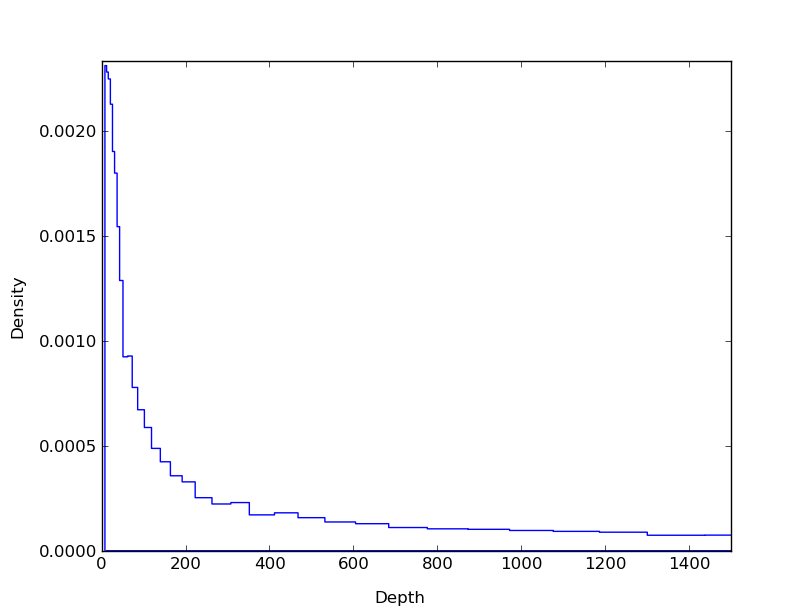
\includegraphics[width=6in]{../media/sdd_financial2_0-1000000.png}
  \caption[SDD of trace Financial2.spc]{This shows the stack depth
  distribution (SDD) for the first 1000000 page requests from Financial1.spc.}
  \label{fig:sdd_financial2}
  \end{figure}

  \begin{figure}
  \centering
  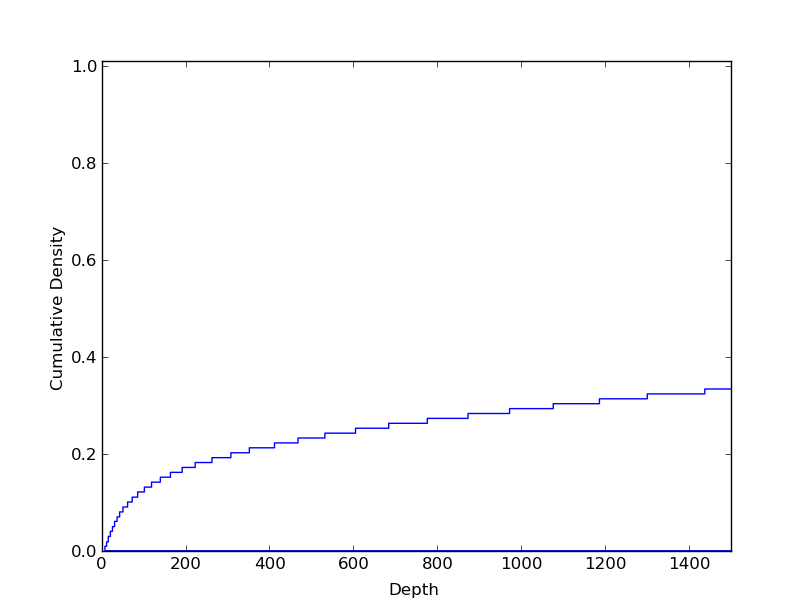
\includegraphics[width=6in]{../media/sdd_cdf_financial2_0-1000000.png}
  \caption[CDF for the SDD of trace Financial2.spc]{This is the cumulative
  distribution function for the stack depth distribution for the first 1000000
  page requests from Financial1.spc. The cumulative value at a depth of 445 is
  12.7\%.}
  \label{fig:sdd_cdf_financial2}
  \end{figure}

  MMC records the relative depth and rank for all pages in cache. Figure
  \ref{fig:ev_1000_financial1} plots these eviction points for all evictions made
  by the two-source MMC algorithm for the first million requests of
  Financial1.spc with a cache that can hold 1000 pages. A few interesting
  features stand out. First, a horizontal line exists at the depth 1000.
  At various points, the value $\tau_1$ is set to the value 1, which is shown in
  Figure \ref{fig:tau_and_theta_1000_financial1}. When $\tau_1 = 1$, the
  algorithm behaves like an LRU. The eviction plot in Figure
  \ref{fig:ev_1000_financial1} also shows two dense eviction regions. These
  correspond to the pages that the algorithm has identified as coming either from
  the independent reference model (this is the region in the top left of the
  graph where the depth of the pages is well over the size of the cache) or from
  the stack depth distribution.

  A small diagonal region at the top right of the graph shows the effect of the
  rolling trace history. When a page is identified as being very important for
  the independent reference model, the algorithm will keep hold of it as long
  as possible. However, the rank of these pages will quickly deteriorate when
  the cluster of references is rolled off the trace.

  A hyperbolically shaped curve exists in Figure \ref{fig:ev_1000_financial1}
  that corresponds to points that could not be cleanly identified as coming from
  the SSD or the IRM. The shape of this curve depends on all of the model
  parameters, but it shows the general relationship that as a page becomes more
  used (i.e., it is highly ranked in the IRM), the algorithm is willing to hold
  onto the page for longer periods of time.

  This graph also shows hints that the mixture model does not have enough
  degrees of freedom to fully capture the memory usage patterns. The most
  obvious issue is the vertical line at rank 1000. If $\tau_2$ were set to 1,
  then MMC would evict pages when their rank exceeds the size of the cache.
  However, as can be seen in Figure \ref{fig:tau_and_theta_1000_financial1},
  $\tau_2$ never equaled 1. Instead, near the end of the trace, the model set
  the value of $\theta_1$ to a very small value that caused the most recent
  pages to be valued so highly that the majority of the distribution was
  essentially flat with an expected value of nearly 0. Since the distribution
  was so flat, the SDD provided very little differentiation between the majority
  of pages. When the value $\theta_1$ was small and $\tau_1$ was not equal to
  1, the relative expected value for pages was determined primarily by
  the IRM.

  \begin{figure}
  \centering
  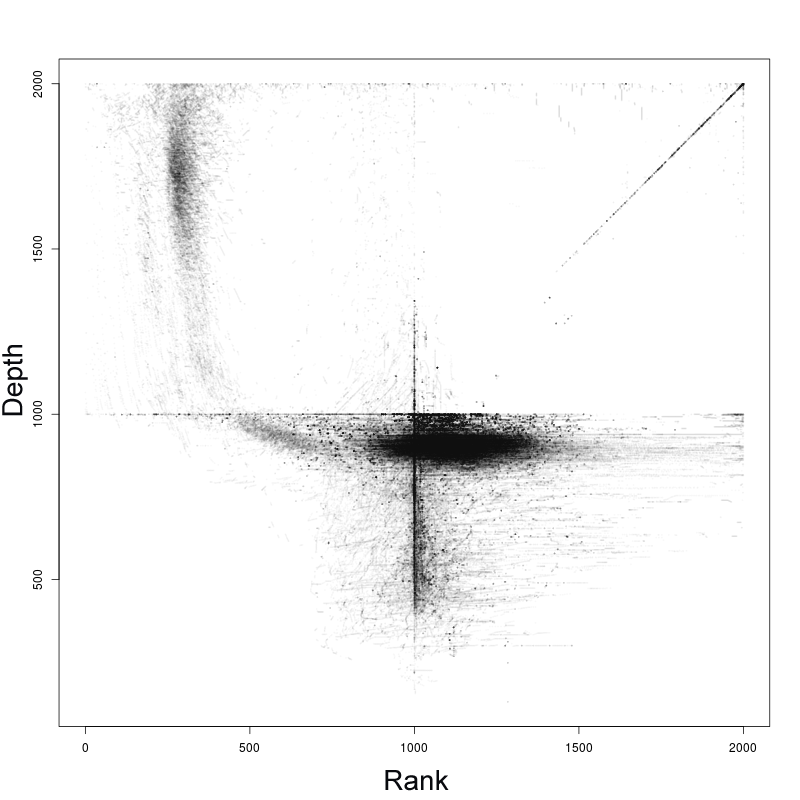
\includegraphics[width=6in]{../media/ev_1000_1000_4000_2.png}
  \caption[Eviction scatterplot for 1000 page MMC cache]{This shows the depth of
  pages in the stack depth distribution (SDD) and the rank of pages in the
  independent reference model (IRM) when they are evicted from the cache by the
  MMC algorithm. The cache can hold 600 pages and can store the metadata for
  another 600 pages. The points in the top right corner represent pages that had
  high rank in the IRM before all of their references rolled off the trace.
  The horizontal line at depth 600 comes from the points in the trace where
  $\tau_1$ equals 1, which causes the algorithm to act like an LRU. The dense
  region in the bottom half of the graph is caused by pages that are assumed to
  be drawn from the SDD. It is denser than the region in the top left of the
  graph because more pages were marked as having come from the SDD than from the
  IRM.}
  \label{fig:ev_1000_financial1}
  \end{figure}

  \begin{figure}
  \centering
  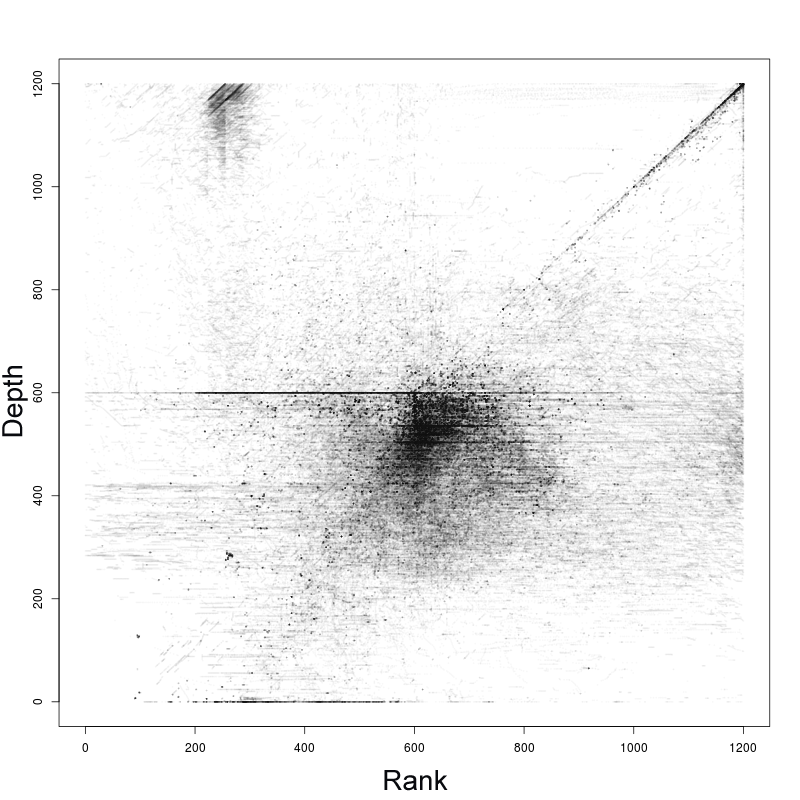
\includegraphics[width=6in]{../media/ev_rw_600_600_2400_2.png}
  \caption[Eviction scatterplot for 1000 page MMC(RW) cache]{This shows the
  depth of pages in the stack depth distribution (SDD) and the rank of pages in
  the independent reference (IRM) model when they are evicted from the cache by
  the MMC(RW) algorithm. The cache can hold 600 pages and can store the
  metadata for another 600 pages. One of the more interesting things about this
  plot is that the algorithm evicted pages with a depth of 0, which means that
  immediately after the pages were requested they were thrown away. When the
  algorithm does not see a request for pages that were recently read or written,
  it decides that the SDD for reads or the SDD for writes is not part of the
  model. Therefore, it assigns a very small expected value to those pages.}
  \label{fig:ev_rw_600_financial1}
  \end{figure}

  \begin{figure}
  \centering
  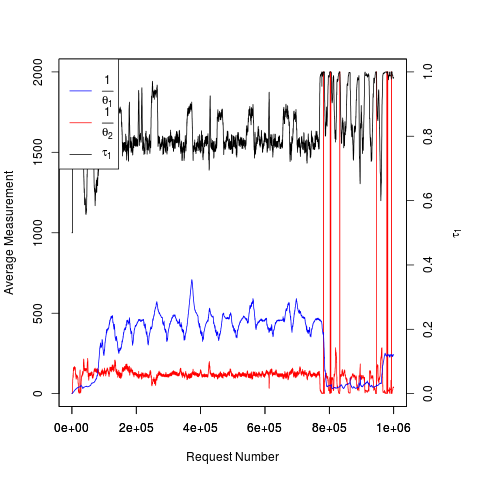
\includegraphics[width=6in]{../media/tau_and_theta_1000_1000_4000_2.png}
  \caption[$\tau_1$, $\frac{1}{\theta_1}$, and $\frac{1}{\theta_2}$ for 1000
  page MMC cache on trace Financial1.spc]
  {This shows all of the model parameters for the two-source MMC
  algorithm with 1000 pages over the first 1000000 page requests on the trace
  Financial1.spc. The value $\tau_1$ ranges between 0 and 1, while the values
  $\frac{1}{\theta_1}$ and $\frac{1}{\theta_2}$ use a scale that shows the
  average value for a page request $X$ drawn from either the SDD modeled with
  $\Geom(H_1(x)|\theta_1)$ or the IRM modeled with $\Geom(H_2(x)|\theta_2)$,
  where the function $H_1$ identifies the depth of page $x$ in the SDD and $H_2$
  identifies the rank of page $x$ in the IRM.}
  \label{fig:tau_and_theta_1000_financial1}
  \end{figure}

  \begin{figure}
  \centering
  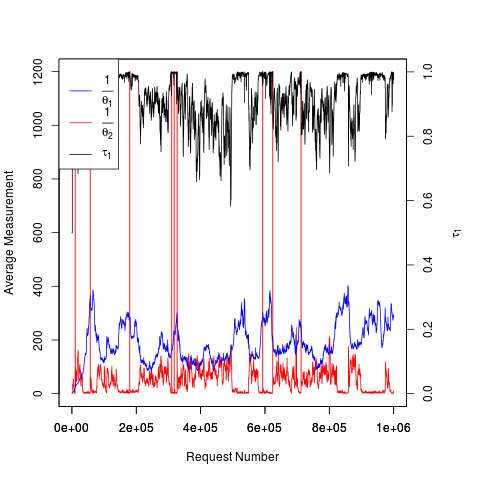
\includegraphics[width=6in]{../media/tau_and_theta_600_600_2400_3.png}
  \caption[$\tau_1$, $\frac{1}{\theta_1}$, and $\frac{1}{\theta_2}$ for 600
  page MMC cache on trace Financial2.spc]{This shows $\tau_1$ for the two-source MMC
  algorithm with 600 pages over the first 1000000 page requests on the trace
  Financial2.spc. When the value of $\tau_1$ is close to 1, MMC behaves much
  like an LRU.}
  \label{fig:tau_and_theta_600_financial2}
  \end{figure}

  We can obtain some insight into how the MMC algorithm works by graphing the
  internal representation of all stored pages. Figure
  \ref{fig:cache_dump_445_financial1} shows a snapshot of the internal
  representation of the pages in the cache. A frozen image doesn't capture the
  dynamic nature of the caching algorithm. The location of pages can change
  drastically after the EM algorithm updates the $\hat{\bm{Z}}$ values for all
  pages. A video showing the internal representation of the pages over time is
  available in the supplemental material \cite{supplimental}.

  \begin{figure}
  \centering
  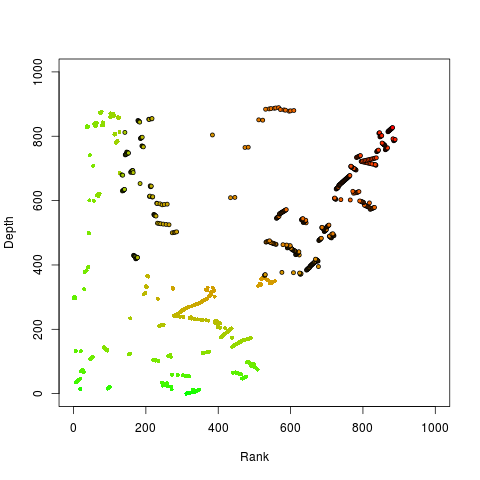
\includegraphics[width=6in]{../media/cache_dump_image_445_445_1780_4_0008090.png}
  \caption[An internal view of a 445 page MMC cache]{This shows a snapshot of
  all pages tracked by the two-source MMC algorithm with 445 pages. Points with
  black circles are evicted pages for which MMC is still storing metadata.}
  \label{fig:cache_dump_445_financial1}
  \end{figure}

